\documentclass{acm_proc_article-sp}

\usepackage{pslatex}
\usepackage{epsfig}
\usepackage{appendix}
\usepackage{float}
\usepackage{url}

\floatstyle{ruled}
\newfloat{program}{thp}{lop}
\floatname{program}{Program}

\begin{document}

\title{Evaluation of Cache-Oblivious Data Structures}
\subtitle{Research Proposal}

\numberofauthors{1}
\author{Maks Verver\\ \email{m.verver@student.utwente.nl}}

% Obligatory permission block
\toappear{
Permission to make digital or hard copies of all or part of this work
for personal or classroom use is granted without fee provided that
copies are not made or distributed for profit or commercial advantage
and that copies bear this notice and the full citation on the first
page. To copy otherwise, or republish, to post on servers or to
redistribute to lists, requires prior specific permission.

\textit{\small 9$^{th}$ Twente Student Conference on IT, Enschede, June, 2008}

Copyright 2008, University of Twente, Faculty of Electrical Engineering,
Mathematics and Computer Science}
% End of obligatory permission block

\maketitle

\begin{abstract}
In modern computer hardware architecture, memory is organized in a hierarchy consisting of several types of memory with different memory sizes, block transfer sizes and access times. The cache-oblivious model has been proposed to reflect this reality more accurately than traditional models. A number of algorithms and data structures have been proposed that perform optimally in this model. The goal of the proposed research project is to implement a selection of cache-oblivious set-like data structures, evaluate their performance (in terms of execution time and memory use) in a realistic environment, and compare their performance to traditional data structures.
\end{abstract}

\keywords{cache efficiency, locality of reference, algorithms}

\section{Introduction}
A fundamental part of theoretical computer science is the study of algorithms (formal descriptions of how computations may be performed) and data structures (descriptions of how information is organized and stored in computers). Traditionally, algorithms have been evaluated in a simplified model of computation. In this model it is assumed that a computer executes an algorithm in discrete steps. At each step it performs one elementary operation (e.g. comparing two numbers, adding one to another, storing a value in memory, et cetera). Each elementary operation is performed within a constant time. In this model, both storing and retrieving data values in memory is considered to be an elementary operation.

This model is close enough to the way computers work to be extremely useful in the development and analysis of data structures and algorithms that work well in practice. However, like every model, it is a simplification of reality. One of the simplifications is the assumption that storing and retrieving data in memory is a constant-time operation (i.e. the uniform memory model). Advancements in software and hardware design over the last two de\-cades have caused this assumption to be increasingly detached from reality.

One of the reasons this assumption fails is that modern operating systems employ virtual memory management, which allows (slower) disk-based storage to be dynamically substituted for (fast\-er) main memory when the latter is in short supply. Another is that as processor speeds have increased greatly, the time required to transfer data between processor and main memory has become a bottleneck for many types of computations. Hardware architects have added faster (but small) cache memory at various points in the computer architecture to reduce this problem, but this increases the differences in access time between different types of memory.

As a result, a modern computer system lacks a central memory storage with uniform performance characteristics. Instead, it employs a hierarchy of memory storage types. Figure \ref{fig-memhier} gives a typical example of such a hierarchy. The processor can directly manipulate data contained in its registers only. To access data in a lower level in the memory hierarchy, the data must be transfered upward through the memory hierarchy. Memory is typically transfered in blocks of data of a fixed size (although bulk transfers involving multiple blocks of data at once are also supported at the memory and disk level).

\begin{figure}
\centering
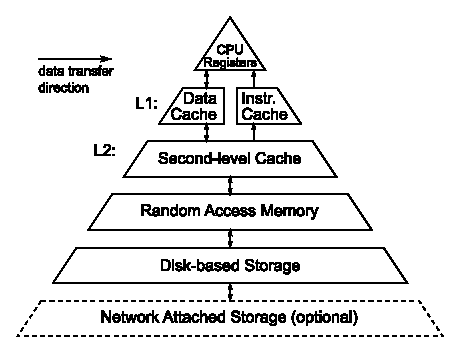
\includegraphics{memhier}
\caption{Schematic depiction of the memory hierarchy}\label{fig-memhier}
\end{figure}

In the memory hierarchy, every next level of storage is both significantly slower and significantly larger than the one above it and with increasing memory sizes, the block size increases as well. Table \ref{tab-memhier} gives an overview of typical memory sizes, block sizes, and access times. The values for the (general purpose) registers, L1 cache and L2 cache are those for the Pentium M processor as given in \cite{intel-opt}; other values are approximate.

\begin{table}
\begin{center}
\begin{tabular}{ l l l l }
\hline
\textbf{Type} & \textbf{Total Size} & \textbf{Block Size} & \textbf{Access Time} \\
\hline
Registers  &   32 bytes & 4 bytes & 1 cycle \\
L1 Cache   &   32 KB    & 64 bytes & 3 cyles \\
L2 Cache   &    1 MB    & 64 bytes & 9 cycles \\
RAM        &   ~2 GB    & 1 KB     & 50-100 cycles \\
Disk       & ~300 GB    & 4 KB     & 5,000-10,000 cycles \\
\hline
\end{tabular}
\caption{Sizes and access times of various types of storage}
\label{tab-memhier}
\end{center}
\end{table}


To conclude: the memory model used in real computer systems is quite a bit more complex than the uniform memory model assumed. Given this reality, the performance of many existing algorithms and data structures can be improved by taking the existence of a memory hierarchy into account. To be able to analyze these algorithms and data structures formally, a different, more realistic model of the cost of accessing data in memory is required.

\subsection{Alternative Memory Models}
In the external memory model, as described by Aggarwal and Vitter \cite{aggarwal1988ioc}, a distinction is made between internal memory (which is limited in size) and external memory (which is virtually unlimited). The external memory is subdivided into blocks of a fixed size and only entire blocks of data can be transferred between the two memories. Although Aggarwal and Vitter focus on magnetic disk as a storage medium for external memory, the model can be generalized to apply to every pair of adjacent levels in the memory hierarchy. In that case, the possibility of transferring several data blocks at once (bulk transfer) may have to be dropped.

The external memory model has the limitation that it only describes two levels of storage, while we have seen that in practice the memory hierarchy is deeper. Even though the external memory model can be used to describe any pair of adjacent levels, a particular algorithm can only be tuned to one. Aggarwal, Alpern, Chandra and Snir \cite{aggarwal1987mhm} introduced a hierarchical memory model in which the cost of accessing a value at specific memory address is described by a non-decreasing function of this address, which means that accessing data at higher addresses can be slower than at lower addresses. This more closely resembles a real memory hierarchy.

We will call algorithms that are designed to minimize the number of transfers in a two-level memory hierarchy ``cache-aware'' (as opposed to traditional ``cache-unaware'' algorithms) or ``cache-conscious''. These algorithms typically rely on knowledge of the block size to achieve optimal performance.

\subsection{Cache-Oblivious Memory Model}
The external memory model was generalized and simplified into the cache-oblivious model \cite{prokop1999coa} which consists of an infinitely large external memory and an internal memory of size M which operates as a cache for the external memory. Data is transferred between the two in aligned data blocks of size B. In this model (and unlike the external memory model) the values of parameters like M and B are not known to algorithms and data structures, so they cannot be referenced explicitly in their definition. Of course, analysis in terms of memory transfers does involve these parameters, so the number of memory transfers performed is still a function of M and B (and other parameters relevant to the problem).

It should be noted that the cache-oblivious model can also be considered similar to the hierarchical model discussed above. The main difference between the two is that in the hierarchical model the application has explicit control over which data are placed at the fastest locations, since these have the lowest addresses, while in the cache-oblivious model the internal memory acts as a transparent cache of the external memory, and the application has no explicit control over which values are kept in the cache. The cache-oblivious model is more realistic in this respect, as applications typically have not explicit control over the cache.

Algorithms that perform optimally in this model are called ``cache-oblivious'' and they distinguish themselves from cache-aware algorithms in that they cannot rely on knowledge of the block size or other specific properties of the cache configuration. The key advantage of this class of algorithms is that they are implicitly tuned to all levels in the memory hierarchy at once. It has been conjectured that these algorithms may therefore perform better than algorithms that are tuned to a specific level in the hierarchy only.

Demaine gives an introduction into the cache-oblivious memory model and an overview of a selection of cache-oblivious data structures and algorithms \cite{demaine2002coa}. He also motivates the simplifications made in the cache-oblivious memory model, such as the assumption of full cache associativity and an optimal replacement policy.

\subsection{Classification}
To summarize the above: data structures and algorithms can be classified by which assumptions they make about the environment. For the purpose of this research project we distinguish between three classes:
\begin{list}{}{}
\item \textbf{Cache-aware} (or \textbf{cache-conscious}) data structures and algorithms perform optimally in the external memory model, but require parametrization with some or all properties of the cache layout (such as block size or cache memory size).
\item \textbf{Cache-unaware} data structures and algorithms are designed with the uniform memory model in mind and may therefore not perform optimally in the external memory model.
\item \textbf{Cache-oblivious} data structures and algorithms are designed to perform optimally in the cache-oblivious model, meaning they are also optimal in the external memory model (in the asymptotic sense and up to a constant factor of memory transfers) without requiring tuning of parameters.
\end{list}

\section{Related Work}
Many data structures and algorithms have been analyzed in the cache-oblivious model. Several new data structures and algorithms have been developed that perform optimally in this mo\-del as well. Prokop presents asymptotically optimal cache-oblivious algorithms for matrix transposition, fast Fourier transformation and sorting \cite{prokop1999coa}.

Bender, Demaine and Farach-Colton designed a cache-oblivious data structure that supports the same operations as a B-tree \cite{bender2005cob} achieving optimal complexity bounds on search and nearly-optimal bounds on insertion. Later, Bender, Duan, Iacono and Wu simplified the data structure \cite{bender2004lpc} while preserving the supported operations and complexity bounds and adding finger searches. The latter data structure consists of a sparse array (stored in a linear amount of memory) with a static search tree in van Emde Boas layout (named after a similar structure proposed by van Emde Boas et al. \cite{vanemdeboas1976dai}).

Askitis and Zobel \cite{askitis2005ccc} propose a way to make chained hash tables more cache-efficient, by storing bucket contents in contiguous memory instead of using a linked list. This means buckets have to be resized on insertions and deletions, but their experiments show a performance gain over traditional methods (especially when the hash table is heavily loaded).

Vitter presents a theoretical survey of algorithms evaluated in a parallel disk model \cite{vitter2001ema}, which is a refinement of the external memory model described by Aggarwal and Vitter, but only allows parallel transfer of multiple blocks from different disks, which is more realistic. Unfortunately, his survey lacks empirical results.

Olsen and Skov evaluated two cache-oblivious priority queue data structures in practice \cite{olsen2002coa} and designed an optimal cache-obli\-vious priority deque. Their main result is that although the cache-obli\-vious data structures they examined make more efficient use of the cache, they do not perform better than traditional priority queue implementations.

\section{Problem Statement}
As described above, several cache-oblivious data structures and algorithms have been proposed. Complexity analysis shows that the proposed solutions are asymptotically optimal. However, in software engineering practice we are not only interested in computational complexity, but also in the practical performance of data structures and algorithms. Indeed, many algorithms that have suboptimal computational complexity are actually widely used because they perform well in practice (for example, sorting algorithms like Quicksort and Shell sort).
%The converse is true as well: some algorithms that are better than widely used alternatives in terms of computational complexity have bad performance on practical data sets, use too much memory, or are too hard to implement correctly (for example, linear time construction of suffix arrays).

This raises the question whether cache-oblivious data structures are actually preferable to traditional data structures in practice. These data structures are designed to perform optimally in a model that was designed to more accurately reflect reality, which suggests they should perform well, but this can only be confirmed by evaluating their performance in a realistic environment and operating on a realistic data set. However, such empirical data is scarce, as existing research has focused mainly on theoretical analysis. The goal of the proposed research project is to perform an empirical evaluation of previously described cache-oblivious data structures and compare them with their traditional counterparts (both cache-aware and cache-unaware data structures).

From the application programmer's point of view, data structures and algorithms can be grouped together based on the functionality they provide. For example, all comparison-based sorting algorithms can be considered to provide equivalent functionality, even if their performance is different. Since it is not sensible to compare data structures which provide different functionality, it is necessary to limit the scope of the project to data structures that provide similar functions. As will be described below, we will limit ourselves to one particular kind of data structures, in the hope that our results may give some insight in the performance of cache-oblivious data structures in general.

\subsection{Research Questions}
Following from the above, the main question to be answered is:
\begin{list}{}{}
\item Do cache-oblivious data structures have practical merit?
\end{list}

Because we are primarily interested in practical performance, actual execution time is the most important metric. Memory use is of interest as well (if only as a secondary criterion) as it may reveal that there is a trade-off between memory use and execution time of data structures. That means that the main question will be answered by first addressing the following questions:
\newcounter{cnt}
\begin{list}{\arabic{cnt}.}{\usecounter{cnt}}
\item How fast are cache-oblivious data structures when compared to cache-aware data structures?
\item How fast are cache-oblivious data structures when compared to cache-unaware data structures?
\item How much memory do cache-oblivious data structures use compared to other data structures?
\end{list}
These questions can be answered by implementing the relevant data structures and measuring their practical performance on a realistic data set.

\section{Research Approach}
The goal of the project is to evaluate a variety of data structures in a practical setting. For this, we need a realistic scenario that makes heavy use of data structures of which cache-oblivious implementations are available. A scenario that suits these needs, is that of a state space search algorithm (or, in short: state search). The purpose of such an algorithm is to find a path from a (set of) given initial state(s) to a goal state. State search algorithms are often used to solve reachability problems, which occur for example in formal model checking. In a simple implementation, such as given in Program \ref{prog-search}, the main data structures used are a queue and a dynamic set.

\begin{program}
\begin{verbatim}
Queue queue = new Queue;
Set visited = new Set;
queue.insert(initial_state);
while (!queue.empty()) {
    State state = queue.extract();
    for (State s : successors(state)) {
        if (isGoal(s)) break;
        if (visited.contains(s) == false) {
            visited.insert(s);
            queue.insert(s);
        }
    }
}
\end{verbatim}
\caption{Pseudo-code for a simple state search algorithm.}
\label{prog-search}
\end{program}

In this program, a queue is a data structure where elements can be inserted and extracted on a first-in-first-out basis. A dynamic set is a data structure that models a set to which elements may be added (and optionally, from which they may be removed) and which may be queried to see if the set contains a particular element.

Since implementing a normal queue is fairly straightforward, the execution time of the algorithm will be dominated by the performance of the set, assuming domain-specific functions (like \verb#isGoal# and \verb#successors# in the sample code) are efficient enough not to dominate the performance of the algorithm. The main focus of the research project will therefore be on alternative implementations of the set data structure.

%The situation changes, of course, when instead of a first-in-first-out queue a priority queue is used. This is often the case when we are searching for a shortest path (instead of any path that reaches the goal) or when heuristics are used in the search. In this case, the complexity of the queue implementation increases. If time allows it, the project could be extended to evaluating different implementations of priority queues as well.

\subsection{Set Operations}
At a minimum, a set data structure should be able to determine whether or not a given element is a member of the set. A dynamic set differs from a static set in that it supports operations to add and/or remove elements from the set dynamically. In our experiments, we will start out with an empty set and only allow for insertion of new elements. This means the our dynamic set must support two basic operations:
\begin{itemize}
\item \verb#insert(S,X)# -- Inserts $X$ into set $S$, if it is not yet present.
\item \verb#contains(S,X)# -- Returns whether set $S$ contains $X$.
\end{itemize}
In practice, it is useful to be able to test if a set contains an element and add this element if it does not. This can be implemented by first testing for the existence, and then conditionally inserting the element (as is done in Program \ref{prog-search}) but many data structures allow to combine this into a single operation. To take advantage of this possibility, we will require that the \verb#insert# operation also returns whether or not the element was newly inserted.

\subsection{Set Implementations}
Many different data structures have been developed that can be used to efficiently implement the operations described above. For each of the categories identified earlier, at least one data structure will be implemented:
\begin{itemize}
\item \textbf{Cache-unaware}: hash tables. Hash tables are widely used in practice and noted for good performance if the data set fits in main memory, although they have also been used as an index structure for data stored on disk. Other possibilities are Patricia trees \cite{morrison1968ppa}, Splay trees \cite{sleator1985sab} or one of the many other variations on search trees.
\item \textbf{Cache-aware}: B-trees. The B-tree is the standard choice for storing ordered data on disk, and depends on a page size being selected that corresponds with the size of data blocks that can be efficiently transferred.
\item \textbf{Cache-oblivious}: the B-tree-like data structure proposed by Bender, Duan, Iacono and Wu. Since it provides functionality comparable to that of a normal B-tree, this seems like a fair candidate for a comparison. An alternative is the cache-oblivious exponential search tree proposed by Rahman, Cole and Raman. \cite{rahman2001opd}.
% The second, if I can find it! (If so, add description to related work)
\end{itemize}

The cache-oblivious data structures have been developed recently and are not commonly used in practice. These will have to be implemented from scratch, using existing publications as a guideline. The traditional data structures are commonly used and therefore have high-quality implementations already available as software libraries. For this research, however, it is undesirable to use existing libraries, for two reasons. First, many existing implementations support additional operations (such as removal of elements, locking and synchronization, atomic transactions, et cetera) which are not used in our experiments, but which may harm the performance of these implementations. Second, many established libraries have been thoroughly optimized while our newly implemented data structures have not. This may give the existing libraries an unfair advantage.

In an attempt to reduce the bias caused by differences in functionality and quality between existing and newly developed libraries, all data structures used in the performance evaluation will be implemented from scratch.

\subsection{Measurement}
As described in the problem statement, the main metric of interest is the total execution time of our algorithm. To be able to quantify the obtained results, we also need to be able to estimate the overhead incurred by the use of our testing framework and other outside influences. Two methods will be employed:
\begin{itemize}
\item Profiling tools such as OProfile \cite{oprofile} can be used to determine which part of the execution time was spent executing the testing framework, with a small overhead during execution.
\item A mock set implementation will be written that does not implement set functionality itself, but gives precomputed answers to queries. This can be used to give an upper bound on the overhead caused by the testing framework.
\end{itemize}

As a secondary metric, we are interested in the memory use of the different data structures. This is harder to quantify, but the following methods may be employed:
\begin{itemize}
\item The maximum resident set size of a process is a lower bound on the amount of memory a process used.
\item The number of times a memory page has to be read from or written to disk is an indication of how often the application exceeds the available main memory.
\end{itemize}
Note that these metrics only given an indication of memory use on the boundary between main memory and disk storage.

\subsection{Test Data}
The test data will be generated with state space generation software that generates synthetic test data based on parameters supplied by the user. This allows us to assess the effect of varying parameters on the performance of the data structures being evaluated. Since the same software is already used in state search related research, the generated test cases are expected to be representative of realistic data sets.

The results may depend on the properties of the generated test data. At least three variables can be identified:
\begin{itemize}
\item The size of the data set: Cache-oblivious data structures usually rely on asymptotic optimality, which means that they may not perform well on small data sets. It would be interesting to see what the effect of various data sizes is on their relative performance.
\item The ratio between queries and insertions: for a particular data structure, it may be much more efficient to query the existence of a value in the set than to add a new value to it. We should either ensure our ratio between queries and insertions is realistic, or run experiments with varying ratios to see how this affects the performance of different data structures.
\item Data access patterns: some data structures perform better when accessing elements that have recently been accessed before. For example, splay trees explicitly support this principle. Again, we should either ensure our access patterns are realistic, or test with varying access patterns and see how data structures are affected.
\end{itemize}

\section{Planning}
\begin{table}
\begin{center}
\begin{tabular}{ | l | l | l | }
\hline
\textbf{Task} & \textbf{Result} & \textbf{Deadline} \\
\hline
Finish proposal
    & Final research proposal
    & March 27th \\
Study literature
    & "Related Work" section
    & April 4th \\
Implement algorithms
    & Working code
    & April 28th \\
Finish paper contents
    & Complete paper
    & May 6th \\
Revise paper
    & Revised paper
    & May 23rd \\
Final paper formatting
    & Finished paper
    & June 11th \\
Prepare presentation
    & Presentation
    & June 20th \\
\hline
\end{tabular}
\caption{Planning}
\label{tab-planning}
\end{center}
\end{table}
See table \ref{tab-planning}.

\bibliographystyle{plain}
\bibliography{proposal}
\end{document}
